\documentclass{article}
\usepackage{amsmath}
\usepackage{graphicx}
\usepackage{geometry}[margin=2cm]
\usepackage{example}
\usepackage{titlesec}

\title{PHY224 Curve Fit Lab 1}
\author{Hachem Fattouh}
\date{\today}

\titleformat{\title}
  {\normalfont\LARGE\bfseries} % Change \LARGE to the desired size, e.g., \large, \Large, \small, etc.
  {}
  {0pt}
  {}

\title{PHY224 Curve Fit Lab 1}
\author{Hachem Fattouh}
\date{\today}

\begin{document}

\maketitle

\begin{figure}[h]
  \centering
  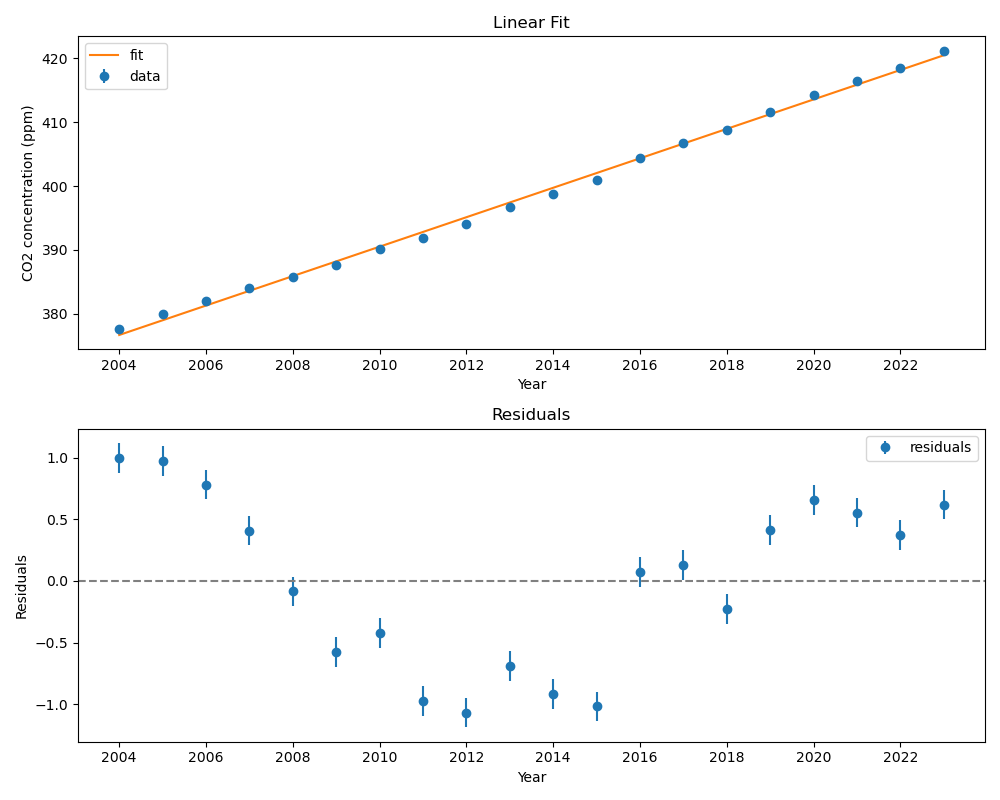
\includegraphics[width=\textwidth]{Exercise 1.png} 
  \caption{the 2 figures above are the linear data with its line of best fit,
  and the corresponding residuals for each dataset.}
  \label{fig:fit_and_residuals}
\end{figure}

in exercise 1, we are given climate data containing the mean atmospheric CO2 content over the last half-century. using this data in a CSV file I plotted the data
for the last 20 years, along with a line of best fit using the linear regression line \(f(x) = ax + b\).


from the data, the coefficients calculated were:
\[a = 2.303\]
\[b = -4239\]
\[r^2 = 0.997\]

from the data, it can also be inferred that in 2060, the atmospheric
CO\textsubscript{2} levels will be 505.18ppm and in 1960 it was
274.88ppm.

\pagebreak

\begin{figure}[h]
  \centering
  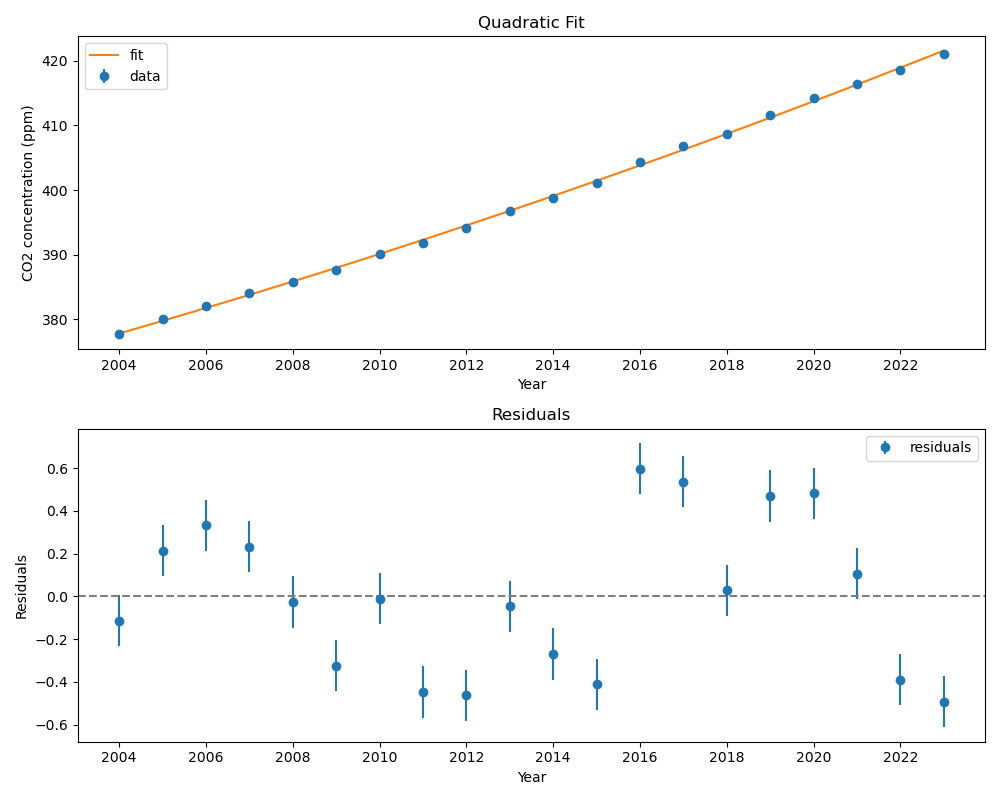
\includegraphics[width=\textwidth]{Exercise 1-2.png} 
  \caption{the 2 figures above are the quadratic data with its line of best fit,
  and the corresponding residuals for each dataset.}
  \label{fig:fit_and_residuals}
\end{figure}

the same data set was then fitted into a quadratic graph with 
equation \(ax^2 + bx + c\) as shown above with values obtained as

\[a = 0.19, b = -76.3, c = 74900.0, \chi^2 = 10.18\]

note that this model is more accurate to reality due to its smaller
$\chi^2$ value. using this new improved model the
data for 2060 and 1960 respectively
is 547 and 330 ppm respectively

\end{document}
